\section{Model selection and additional diagnostics}

\subsection{PINN architecture and optimization screening}
\label{app:tuning}

The final PINN configuration was obtained by a staged sensitivity study, not by optimizing on the final six-budget table. Each recorded development run used Tests 1--4, budgets \(N\in\{50,200\}\), seeds 101--103, and 5,000 epochs unless stated otherwise. At each stage we inspected interpolation and extrapolation primary \(R^2\), RMSE, physics-validation residuals, run-to-run variation, and cost. A candidate was retained before moving to the next stage. This procedure is substantially cheaper than the full Cartesian product, but it does not estimate interactions between all hyperparameters.

Table~\ref{tab:pinn_screen} lists the candidate sets reconstructed from the stored experiment namespaces and checkpoint metadata. The gated residual backbone with width 128 and six hidden layers was fixed before the recorded comparison. In particular, only this width/depth pair survives in the unified experiment archive; we therefore do not claim a systematic width/depth grid search. The activation comparison was complete for tanh, SiLU, and GELU, and GELU had the strongest pooled primary \(R^2\) across the development rows. The later stages retained \(L^0_{\mathrm{data}}=0.03\), \(L^0_{\mathrm{ibc}}=0.003\), HO floor \(c=0.25\), \(N_r/N=2\), and initial learning rate \(3\times10^{-3}\). Training was then extended from 5,000 to 10,000 epochs.

\begin{table*}[!htbp]
\centering
\small
\setlength{\tabcolsep}{3pt}
\caption{Recorded sequential PINN screening. Values in bold are used in the final experiments. The gate search was staged, so the listed values were not evaluated as one Cartesian product.}
\label{tab:pinn_screen}
\begin{tabular}{p{0.19\textwidth}p{0.52\textwidth}p{0.20\textwidth}}
\toprule
Stage & Values represented in completed experiment namespaces & Retained value\\
\midrule
Backbone size & Width 128, depth 6; no completed alternative width/depth grid in the unified archive & \textbf{128 / 6}\\
Activation & tanh, SiLU, GELU, with H-PINN and HO-PINN & \textbf{GELU}\\
Data gate target & \(L^0_{\mathrm{data}}\in\{0.01,0.03,0.1,0.3\}\) across staged runs & \textbf{0.03}\\
IBC gate target & \(L^0_{\mathrm{ibc}}\in\{0.001,0.003,0.01,0.03\}\) across staged runs & \textbf{0.003}\\
HO orthogonal floor & \(c\in\{0,0.25,0.5,0.75,1\}\); \(c=1\) is H-PINN weighting & \textbf{0.25}\\
Residual density & \(N_r/N\in\{1,2,4\}\), freshly resampled each epoch & \textbf{2}\\
Initial learning rate & \(\{3\times10^{-4},3\times10^{-3},10^{-2}\}\), cosine decay to \(10^{-5}\) & \textbf{\(3\times10^{-3}\)}\\
Epoch budget & 5,000 in screening; 10,000 in the reported runs & \textbf{10,000}\\
Optimizer and checkpoint & Adam; gradient clipping at 1; minimum detached balanced training loss & \textbf{fixed}\\
\bottomrule
\end{tabular}
\end{table*}

The stored activation runs give pooled development primary \(R^2\) values of 0.575, 0.596, and 0.618 for tanh, SiLU, and GELU, respectively, when averaging both PINN variants, all four tests, both regions, both development budgets, and three seeds. These pooled numbers are diagnostic only: they mix tasks with different response ranges and were never reported as a scientific performance metric. For the HO floor, the corresponding pooled values are 0.657, 0.658, 0.654, 0.657, and 0.655 for \(c=0,0.25,0.5,0.75,1\), showing that the choice of 0.25 is a shallow optimum rather than a decisive effect.

Selection of the gate targets was based on joint inspection rather than a preregistered scalar objective. For example, \(L^0_{\mathrm{ibc}}=0.001\) gives a slightly higher pooled development primary \(R^2\) than 0.003, while 0.003 was retained as the compromise used in the subsequent residual-density and learning-rate studies. We report this detail because choosing a retrospective scalar aggregation would overstate the precision of the tuning procedure. The final values should be interpreted as one robust common configuration, not a proof that each scalar is globally optimal.

The numerical seeds 101--103 were reused in the final table. The flow reference solutions were subsequently replaced by the corrected conservative generator, and the selected configuration was not retuned per corrected flow test, per budget, or per region. This reduces direct adaptation to Tests 2--4 but does not create an independent confirmatory seed set. Future work should repeat the frozen configuration on additional seeds and independently generated permeability fields.

\subsection{Classical-baseline hyperparameter searches}

Every classical candidate is fitted only on the current labelled set. Tests 2--4 use three strictly forward expanding-window folds; each validation block is later than its training block. Searches are performed independently for pressure, oil saturation, and water saturation, with negative MSE as the selection score. Input scaling and, for strong-profile SVR, target scaling are fitted within each fold.

\begin{table*}[!htbp]
\centering
\small
\setlength{\tabcolsep}{3pt}
\caption{Classical search spaces. The strong profile is used for Tests 2--4 at every budget and seed. Test 1 uses the standard profile described in the last row.}
\label{tab:classical_search}
\begin{tabular}{p{0.12\textwidth}p{0.69\textwidth}p{0.12\textwidth}}
\toprule
Method & Strong-profile candidates & Evaluated\\
\midrule
XGB & \(n_{\rm est}\in\{100,300,600,1000\}\), depth \(\in\{2,3,4,6\}\), learning rate \(\in\{0.01,0.03,0.05,0.1\}\), child weight \(\in\{1,3,5\}\), subsample \(\in\{0.7,0.85,1\}\), feature fraction \(\in\{0.7,0.9,1\}\), \(\ell_1\in\{0,0.01,0.1\}\), \(\ell_2\in\{0.1,1,10\}\) & 32 random\\
RBF-SVR & \(C\in\{0.1,1,10,100,1000\}\), \(\gamma\in\{\text{scale},\text{auto},0.01,0.03,0.1,0.3,1,3,10\}\), \(\epsilon\in\{10^{-4},10^{-3},10^{-2},0.03,0.05,0.1\}\) & 40 random\\
GP & Constant-scaled RBF, Mat\'ern-3/2, Mat\'ern-5/2, or rational-quadratic kernel, each with white noise; nugget \(\alpha\in\{10^{-8},10^{-6},10^{-4}\}\) & 12 grid\\
Test 1 & XGB: \(2\times2\times2=8\) estimator/depth/rate combinations; SVR: \(3\times3=9\) \(C/\gamma\) combinations with \(\epsilon=10^{-3}\); anisotropic RBF GP optimized by marginal likelihood & standard\\
\bottomrule
\end{tabular}
\end{table*}

The selected parameter dictionary, fold count, candidate count, and cross-validation score are serialized in each classical result row. Consequently, ``training-only tuned'' means that hyperparameters were selected inside the labelled training subset; it does not mean that defaults were used. Neither interpolation nor extrapolation evaluation values enter these searches.

\subsection{Complete primary comparison}
\label{app:primary_tables}

Tables~\ref{tab:primary_full_n20} and \ref{tab:primary_full_n100} report all five methods at the two budgets summarized in Table~\ref{tab:primary_summary}. They are separated by budget to preserve a normal reading orientation and a legible numerical font.

\begin{table*}[t]
\centering
\scriptsize
\setlength{\tabcolsep}{3.2pt}
\caption{Complete primary $R^2$ comparison at $N=20$ (mean $\pm$ sample standard deviation over seeds 101--103). Test 1 uses temperature; Tests 2--4 use water saturation. Bold marks the highest mean in each row.}
\label{tab:primary_full_n20}
\begin{tabular}{@{}llccccc@{}}
\toprule
Test & Region & H-PINN & HO-PINN & XGB & SVR & GP \\
\midrule
T1 & Interp. & \textbf{$0.997\pm0.002$} & $0.997\pm0.002$ & $0.314\pm0.195$ & $0.431\pm0.132$ & $0.775\pm0.132$ \\
T1 & Forecast & \textbf{$0.955\pm0.016$} & $0.936\pm0.030$ & $0.254\pm0.323$ & $0.395\pm0.363$ & $-0.015\pm0.552$ \\
\addlinespace[1pt]
T2 & Interp. & $0.900\pm0.038$ & \textbf{$0.901\pm0.038$} & $0.375\pm0.033$ & $0.417\pm0.158$ & $0.564\pm0.105$ \\
T2 & Forecast & \textbf{$0.834\pm0.027$} & $0.828\pm0.034$ & $0.143\pm0.191$ & $-0.171\pm0.361$ & $0.063\pm0.362$ \\
\addlinespace[1pt]
T3 & Interp. & $0.567\pm0.031$ & \textbf{$0.576\pm0.027$} & $0.125\pm0.049$ & $0.204\pm0.076$ & $-0.038\pm0.641$ \\
T3 & Forecast & $0.547\pm0.051$ & \textbf{$0.547\pm0.041$} & $0.070\pm0.088$ & $-1.344\pm2.152$ & $0.056\pm0.416$ \\
\addlinespace[1pt]
T4 & Interp. & \textbf{$0.517\pm0.044$} & $0.516\pm0.044$ & $-0.189\pm0.346$ & $-0.199\pm0.497$ & $0.058\pm0.129$ \\
T4 & Forecast & $0.632\pm0.017$ & \textbf{$0.632\pm0.019$} & $-0.009\pm0.330$ & $-0.271\pm0.520$ & $-0.126\pm0.226$ \\
\bottomrule
\end{tabular}
\end{table*}

\begin{table*}[t]
\centering
\scriptsize
\setlength{\tabcolsep}{3.2pt}
\caption{Complete primary $R^2$ comparison at $N=100$ (mean $\pm$ sample standard deviation over seeds 101--103). Test 1 uses temperature; Tests 2--4 use water saturation. Bold marks the highest mean in each row.}
\label{tab:primary_full_n100}
\begin{tabular}{@{}llccccc@{}}
\toprule
Test & Region & H-PINN & HO-PINN & XGB & SVR & GP \\
\midrule
T1 & Interp. & \textbf{$1.000\pm0.000$} & $0.999\pm0.001$ & $0.847\pm0.043$ & $0.993\pm0.004$ & \textbf{$1.000\pm0.000$} \\
T1 & Forecast & \textbf{$0.969\pm0.009$} & $0.943\pm0.038$ & $0.584\pm0.121$ & $0.645\pm0.180$ & $-0.168\pm0.441$ \\
\addlinespace[1pt]
T2 & Interp. & \textbf{$0.977\pm0.009$} & $0.975\pm0.009$ & $0.741\pm0.047$ & $0.816\pm0.040$ & $0.859\pm0.045$ \\
T2 & Forecast & $0.933\pm0.011$ & \textbf{$0.933\pm0.014$} & $0.460\pm0.030$ & $0.579\pm0.171$ & $0.511\pm0.084$ \\
\addlinespace[1pt]
T3 & Interp. & \textbf{$0.840\pm0.014$} & $0.836\pm0.022$ & $0.666\pm0.041$ & $0.616\pm0.035$ & $0.745\pm0.052$ \\
T3 & Forecast & \textbf{$0.780\pm0.052$} & $0.771\pm0.055$ & $0.491\pm0.072$ & $-1.021\pm1.095$ & $0.483\pm0.126$ \\
\addlinespace[1pt]
T4 & Interp. & $0.715\pm0.008$ & \textbf{$0.720\pm0.017$} & $0.474\pm0.108$ & $0.258\pm0.052$ & $0.466\pm0.266$ \\
T4 & Forecast & $0.725\pm0.037$ & \textbf{$0.737\pm0.038$} & $0.353\pm0.116$ & $0.212\pm0.102$ & $0.262\pm0.419$ \\
\bottomrule
\end{tabular}
\end{table*}


\subsection{Additional error and physical metrics}
\label{app:additional_metrics}

The main text reports target-resolved MSE and \(R^2\). Table~\ref{tab:test1_secondary} and Tables~\ref{tab:secondary_test2}--\ref{tab:secondary_test4} add RMSE, MAE, relative \(L^2\), and standard-deviation-normalized RMSE at \(N=50\). The definitions are
\begin{align}
\mathrm{RMSE}&=\sqrt{\mathrm{MSE}},
&\mathrm{MAE}&=\frac1m\sum_i|y_i-\widehat y_i|,\\
\mathrm{relative}\ L^2&=\frac{\lVert\boldsymbol y-\widehat{\boldsymbol y}\rVert_2}{\lVert\boldsymbol y\rVert_2},
&\mathrm{NRMSE}_{\mathrm{std}}&=\frac{\mathrm{RMSE}}{\operatorname{std}(\boldsymbol y)}.
\end{align}
The oil-saturation results and every seed-level value remain in the machine-readable \texttt{final\_results\_used.csv}; duplicating all six budgets and all three flow targets in print would obscure rather than clarify the primary comparison.

\begin{table*}[!htbp]
\centering
\small
\setlength{\tabcolsep}{3.2pt}
\caption{Complete Test 1 metrics at $N=50$ (mean $\pm$ sample standard deviation over seeds 101--103).}
\label{tab:test1_secondary}
\textbf{(a) Absolute errors}\par\smallskip
\begin{tabular}{llccc}
\toprule
Region & Method & MSE & RMSE & MAE \\
\midrule
Interp. & H-PINN & $\num{2.12e-04}\,\pm\,\num{1.62e-04}$ & 0.0139\,$\pm$\,0.0053 & 0.0093\,$\pm$\,0.0035 \\
Interp. & HO-PINN & $\num{2.27e-04}\,\pm\,\num{2.02e-04}$ & 0.0141\,$\pm$\,0.0063 & 0.0091\,$\pm$\,0.0039 \\
Interp. & XGB & $\num{5.10e-02}\,\pm\,\num{1.53e-02}$ & 0.2242\,$\pm$\,0.0335 & 0.1273\,$\pm$\,0.0142 \\
Interp. & SVM & $\num{1.16e-02}\,\pm\,\num{2.92e-03}$ & 0.1072\,$\pm$\,0.0138 & 0.0400\,$\pm$\,0.0061 \\
Interp. & GP & $\num{5.71e-03}\,\pm\,\num{5.72e-03}$ & 0.0696\,$\pm$\,0.0360 & 0.0252\,$\pm$\,0.0098 \\
\midrule
Extrap. & H-PINN & $\num{5.14e-04}\,\pm\,\num{2.58e-04}$ & 0.0221\,$\pm$\,0.0064 & 0.0139\,$\pm$\,0.0040 \\
Extrap. & HO-PINN & $\num{1.02e-03}\,\pm\,\num{6.87e-04}$ & 0.0308\,$\pm$\,0.0105 & 0.0190\,$\pm$\,0.0064 \\
Extrap. & XGB & $\num{1.26e-02}\,\pm\,\num{2.89e-03}$ & 0.1119\,$\pm$\,0.0132 & 0.0943\,$\pm$\,0.0128 \\
Extrap. & SVM & $\num{1.11e-02}\,\pm\,\num{7.97e-03}$ & 0.1014\,$\pm$\,0.0359 & 0.0827\,$\pm$\,0.0294 \\
Extrap. & GP & $\num{8.33e-03}\,\pm\,\num{7.55e-03}$ & 0.0856\,$\pm$\,0.0390 & 0.0651\,$\pm$\,0.0302 \\
\bottomrule
\end{tabular}
\par\medskip
\textbf{(b) Coefficient of determination and normalized errors}\par\smallskip
\begin{tabular}{llccc}
\toprule
Region & Method & $R^2$ & relative $L^2$ & NRMSE$_{\mathrm{std}}$ \\
\midrule
Interp. & H-PINN & 0.9990\,$\pm$\,0.0007 & 0.0068\,$\pm$\,0.0026 & 0.0299\,$\pm$\,0.0113 \\
Interp. & HO-PINN & 0.9990\,$\pm$\,0.0009 & 0.0069\,$\pm$\,0.0031 & 0.0304\,$\pm$\,0.0136 \\
Interp. & XGB & 0.7649\,$\pm$\,0.0706 & 0.1091\,$\pm$\,0.0163 & 0.4813\,$\pm$\,0.0719 \\
Interp. & SVM & 0.9464\,$\pm$\,0.0135 & 0.0522\,$\pm$\,0.0067 & 0.2302\,$\pm$\,0.0295 \\
Interp. & GP & 0.9737\,$\pm$\,0.0264 & 0.0339\,$\pm$\,0.0175 & 0.1495\,$\pm$\,0.0772 \\
\midrule
Extrap. & H-PINN & 0.9717\,$\pm$\,0.0142 & 0.0110\,$\pm$\,0.0032 & 0.1636\,$\pm$\,0.0473 \\
Extrap. & HO-PINN & 0.9439\,$\pm$\,0.0378 & 0.0153\,$\pm$\,0.0052 & 0.2282\,$\pm$\,0.0777 \\
Extrap. & XGB & 0.3049\,$\pm$\,0.1590 & 0.0558\,$\pm$\,0.0066 & 0.8299\,$\pm$\,0.0979 \\
Extrap. & SVM & 0.3874\,$\pm$\,0.4383 & 0.0506\,$\pm$\,0.0179 & 0.7519\,$\pm$\,0.2664 \\
Extrap. & GP & 0.5417\,$\pm$\,0.4154 & 0.0427\,$\pm$\,0.0195 & 0.6345\,$\pm$\,0.2893 \\
\bottomrule
\end{tabular}
\end{table*}

\begin{table*}[t]
\centering
\scriptsize
\setlength{\tabcolsep}{2.7pt}
\caption{Secondary error metrics for Test 2 at $N=50$ (mean $\pm$ sample standard deviation over seeds 101--103).}
\label{tab:secondary_test2}
\begin{tabular}{@{}cllcccc@{}}
\toprule
Target & Region & Method & RMSE & MAE & Relative $L^2$ & NRMSE$_{\rm std}$ \\
\midrule
$p$ & Interp. & H & $0.0062\pm0.0019$ & $0.0034\pm0.0007$ & $0.0101\pm0.0031$ & $0.0178\pm0.0055$ \\
$p$ & Interp. & HO & $0.0059\pm0.0016$ & $0.0033\pm0.0005$ & $0.0097\pm0.0026$ & $0.0170\pm0.0045$ \\
$p$ & Interp. & XGB & $0.0582\pm0.0100$ & $0.0431\pm0.0069$ & $0.0947\pm0.0163$ & $0.1666\pm0.0287$ \\
$p$ & Interp. & SVR & $0.0696\pm0.0029$ & $0.0577\pm0.0024$ & $0.1132\pm0.0047$ & $0.1993\pm0.0082$ \\
$p$ & Interp. & GP & $0.0172\pm0.0032$ & $0.0117\pm0.0013$ & $0.0280\pm0.0053$ & $0.0493\pm0.0093$ \\
\addlinespace[1pt]
$p$ & Forecast & H & $0.0124\pm0.0019$ & $0.0088\pm0.0012$ & $0.0193\pm0.0030$ & $0.0347\pm0.0053$ \\
$p$ & Forecast & HO & $0.0118\pm0.0012$ & $0.0085\pm0.0009$ & $0.0183\pm0.0018$ & $0.0328\pm0.0033$ \\
$p$ & Forecast & XGB & $0.0566\pm0.0053$ & $0.0419\pm0.0033$ & $0.0880\pm0.0082$ & $0.1580\pm0.0147$ \\
$p$ & Forecast & SVR & $0.1050\pm0.0303$ & $0.0860\pm0.0271$ & $0.1632\pm0.0472$ & $0.2930\pm0.0847$ \\
$p$ & Forecast & GP & $0.0245\pm0.0054$ & $0.0183\pm0.0034$ & $0.0381\pm0.0085$ & $0.0685\pm0.0152$ \\
\addlinespace[1pt]
\midrule
$S_w$ & Interp. & H & $0.0360\pm0.0089$ & $0.0151\pm0.0043$ & $0.2014\pm0.0499$ & $0.2305\pm0.0571$ \\
$S_w$ & Interp. & HO & $0.0347\pm0.0075$ & $0.0144\pm0.0035$ & $0.1944\pm0.0422$ & $0.2225\pm0.0483$ \\
$S_w$ & Interp. & XGB & $0.0887\pm0.0047$ & $0.0620\pm0.0056$ & $0.4968\pm0.0266$ & $0.5684\pm0.0304$ \\
$S_w$ & Interp. & SVR & $0.0725\pm0.0081$ & $0.0500\pm0.0037$ & $0.4060\pm0.0456$ & $0.4646\pm0.0522$ \\
$S_w$ & Interp. & GP & $0.0706\pm0.0091$ & $0.0469\pm0.0047$ & $0.3958\pm0.0511$ & $0.4528\pm0.0585$ \\
\addlinespace[1pt]
$S_w$ & Forecast & H & $0.0652\pm0.0108$ & $0.0420\pm0.0082$ & $0.2275\pm0.0376$ & $0.3510\pm0.0580$ \\
$S_w$ & Forecast & HO & $0.0649\pm0.0109$ & $0.0408\pm0.0076$ & $0.2265\pm0.0379$ & $0.3494\pm0.0584$ \\
$S_w$ & Forecast & XGB & $0.1267\pm0.0060$ & $0.1010\pm0.0080$ & $0.4418\pm0.0209$ & $0.6817\pm0.0322$ \\
$S_w$ & Forecast & SVR & $0.1451\pm0.0170$ & $0.1171\pm0.0172$ & $0.5061\pm0.0594$ & $0.7809\pm0.0917$ \\
$S_w$ & Forecast & GP & $0.1193\pm0.0316$ & $0.0919\pm0.0264$ & $0.4160\pm0.1101$ & $0.6418\pm0.1699$ \\
\addlinespace[1pt]
\bottomrule
\end{tabular}
\end{table*}

\begin{table*}[t]
\centering
\scriptsize
\setlength{\tabcolsep}{2.7pt}
\caption{Secondary error metrics for Test 3 at $N=50$ (mean $\pm$ sample standard deviation over seeds 101--103).}
\label{tab:secondary_test3}
\begin{tabular}{@{}cllcccc@{}}
\toprule
Target & Region & Method & RMSE & MAE & Relative $L^2$ & NRMSE$_{\rm std}$ \\
\midrule
$p$ & Interp. & H & $0.0283\pm0.0032$ & $0.0211\pm0.0019$ & $0.0532\pm0.0060$ & $0.0946\pm0.0107$ \\
$p$ & Interp. & HO & $0.0282\pm0.0042$ & $0.0209\pm0.0024$ & $0.0530\pm0.0078$ & $0.0944\pm0.0139$ \\
$p$ & Interp. & XGB & $0.0973\pm0.0067$ & $0.0728\pm0.0009$ & $0.1830\pm0.0126$ & $0.3258\pm0.0225$ \\
$p$ & Interp. & SVR & $0.1154\pm0.0068$ & $0.0899\pm0.0040$ & $0.2170\pm0.0128$ & $0.3863\pm0.0228$ \\
$p$ & Interp. & GP & $0.0539\pm0.0174$ & $0.0355\pm0.0107$ & $0.1014\pm0.0327$ & $0.1806\pm0.0582$ \\
\addlinespace[1pt]
$p$ & Forecast & H & $0.0449\pm0.0058$ & $0.0339\pm0.0044$ & $0.0781\pm0.0102$ & $0.1451\pm0.0189$ \\
$p$ & Forecast & HO & $0.0445\pm0.0049$ & $0.0338\pm0.0035$ & $0.0775\pm0.0084$ & $0.1440\pm0.0157$ \\
$p$ & Forecast & XGB & $0.0949\pm0.0072$ & $0.0737\pm0.0008$ & $0.1653\pm0.0125$ & $0.3073\pm0.0232$ \\
$p$ & Forecast & SVR & $0.1528\pm0.0331$ & $0.1251\pm0.0336$ & $0.2659\pm0.0576$ & $0.4943\pm0.1070$ \\
$p$ & Forecast & GP & $0.0639\pm0.0126$ & $0.0460\pm0.0079$ & $0.1112\pm0.0220$ & $0.2067\pm0.0408$ \\
\addlinespace[1pt]
\midrule
$S_w$ & Interp. & H & $0.0655\pm0.0028$ & $0.0316\pm0.0017$ & $0.4990\pm0.0214$ & $0.5350\pm0.0229$ \\
$S_w$ & Interp. & HO & $0.0651\pm0.0038$ & $0.0314\pm0.0022$ & $0.4961\pm0.0293$ & $0.5319\pm0.0314$ \\
$S_w$ & Interp. & XGB & $0.1082\pm0.0162$ & $0.0579\pm0.0030$ & $0.8243\pm0.1234$ & $0.8838\pm0.1323$ \\
$S_w$ & Interp. & SVR & $0.1036\pm0.0284$ & $0.0641\pm0.0189$ & $0.7891\pm0.2168$ & $0.8460\pm0.2324$ \\
$S_w$ & Interp. & GP & $0.0797\pm0.0179$ & $0.0422\pm0.0044$ & $0.6072\pm0.1361$ & $0.6510\pm0.1459$ \\
\addlinespace[1pt]
$S_w$ & Forecast & H & $0.0993\pm0.0049$ & $0.0617\pm0.0025$ & $0.4799\pm0.0237$ & $0.5853\pm0.0289$ \\
$S_w$ & Forecast & HO & $0.0996\pm0.0065$ & $0.0621\pm0.0041$ & $0.4816\pm0.0317$ & $0.5874\pm0.0386$ \\
$S_w$ & Forecast & XGB & $0.1669\pm0.0253$ & $0.1400\pm0.0275$ & $0.8069\pm0.1222$ & $0.9841\pm0.1491$ \\
$S_w$ & Forecast & SVR & $0.2690\pm0.1703$ & $0.2208\pm0.1448$ & $1.3001\pm0.8232$ & $1.5857\pm1.0040$ \\
$S_w$ & Forecast & GP & $0.1227\pm0.0177$ & $0.0940\pm0.0129$ & $0.5930\pm0.0856$ & $0.7233\pm0.1044$ \\
\addlinespace[1pt]
\bottomrule
\end{tabular}
\end{table*}

\begin{table*}[t]
\centering
\scriptsize
\setlength{\tabcolsep}{2.7pt}
\caption{Secondary error metrics for Test 4 at $N=50$ (mean $\pm$ sample standard deviation over seeds 101--103).}
\label{tab:secondary_test4}
\begin{tabular}{@{}cllcccc@{}}
\toprule
Target & Region & Method & RMSE & MAE & Relative $L^2$ & NRMSE$_{\rm std}$ \\
\midrule
$p$ & Interp. & H & $0.0161\pm0.0037$ & $0.0104\pm0.0025$ & $0.0258\pm0.0059$ & $0.0434\pm0.0100$ \\
$p$ & Interp. & HO & $0.0164\pm0.0034$ & $0.0105\pm0.0023$ & $0.0264\pm0.0055$ & $0.0444\pm0.0092$ \\
$p$ & Interp. & XGB & $0.1072\pm0.0108$ & $0.0780\pm0.0044$ & $0.1723\pm0.0173$ & $0.2893\pm0.0291$ \\
$p$ & Interp. & SVR & $0.1401\pm0.0241$ & $0.1045\pm0.0186$ & $0.2251\pm0.0388$ & $0.3779\pm0.0652$ \\
$p$ & Interp. & GP & $0.0316\pm0.0048$ & $0.0209\pm0.0028$ & $0.0507\pm0.0078$ & $0.0852\pm0.0130$ \\
\addlinespace[1pt]
$p$ & Forecast & H & $0.0231\pm0.0040$ & $0.0148\pm0.0027$ & $0.0365\pm0.0064$ & $0.0611\pm0.0107$ \\
$p$ & Forecast & HO & $0.0223\pm0.0040$ & $0.0143\pm0.0025$ & $0.0353\pm0.0064$ & $0.0591\pm0.0107$ \\
$p$ & Forecast & XGB & $0.1061\pm0.0105$ & $0.0792\pm0.0028$ & $0.1679\pm0.0166$ & $0.2814\pm0.0278$ \\
$p$ & Forecast & SVR & $0.1740\pm0.0655$ & $0.1335\pm0.0523$ & $0.2753\pm0.1036$ & $0.4614\pm0.1736$ \\
$p$ & Forecast & GP & $0.0344\pm0.0056$ & $0.0239\pm0.0035$ & $0.0544\pm0.0089$ & $0.0911\pm0.0150$ \\
\addlinespace[1pt]
\midrule
$S_w$ & Interp. & H & $0.0661\pm0.0028$ & $0.0281\pm0.0018$ & $0.5666\pm0.0236$ & $0.6056\pm0.0253$ \\
$S_w$ & Interp. & HO & $0.0662\pm0.0025$ & $0.0280\pm0.0017$ & $0.5681\pm0.0215$ & $0.6073\pm0.0230$ \\
$S_w$ & Interp. & XGB & $0.0920\pm0.0038$ & $0.0519\pm0.0071$ & $0.7889\pm0.0325$ & $0.8433\pm0.0347$ \\
$S_w$ & Interp. & SVR & $0.1041\pm0.0073$ & $0.0694\pm0.0094$ & $0.8925\pm0.0625$ & $0.9541\pm0.0668$ \\
$S_w$ & Interp. & GP & $0.0884\pm0.0037$ & $0.0454\pm0.0084$ & $0.7582\pm0.0318$ & $0.8105\pm0.0340$ \\
\addlinespace[1pt]
$S_w$ & Forecast & H & $0.0919\pm0.0057$ & $0.0557\pm0.0044$ & $0.4687\pm0.0288$ & $0.5653\pm0.0347$ \\
$S_w$ & Forecast & HO & $0.0930\pm0.0047$ & $0.0561\pm0.0039$ & $0.4738\pm0.0242$ & $0.5715\pm0.0291$ \\
$S_w$ & Forecast & XGB & $0.1327\pm0.0102$ & $0.0928\pm0.0135$ & $0.6765\pm0.0520$ & $0.8160\pm0.0627$ \\
$S_w$ & Forecast & SVR & $0.1665\pm0.0090$ & $0.1211\pm0.0024$ & $0.8485\pm0.0458$ & $1.0234\pm0.0553$ \\
$S_w$ & Forecast & GP & $0.1408\pm0.0211$ & $0.0928\pm0.0129$ & $0.7177\pm0.1074$ & $0.8657\pm0.1296$ \\
\addlinespace[1pt]
\bottomrule
\end{tabular}
\end{table*}


\FloatBarrier
\clearpage

\begin{strip}
\centering
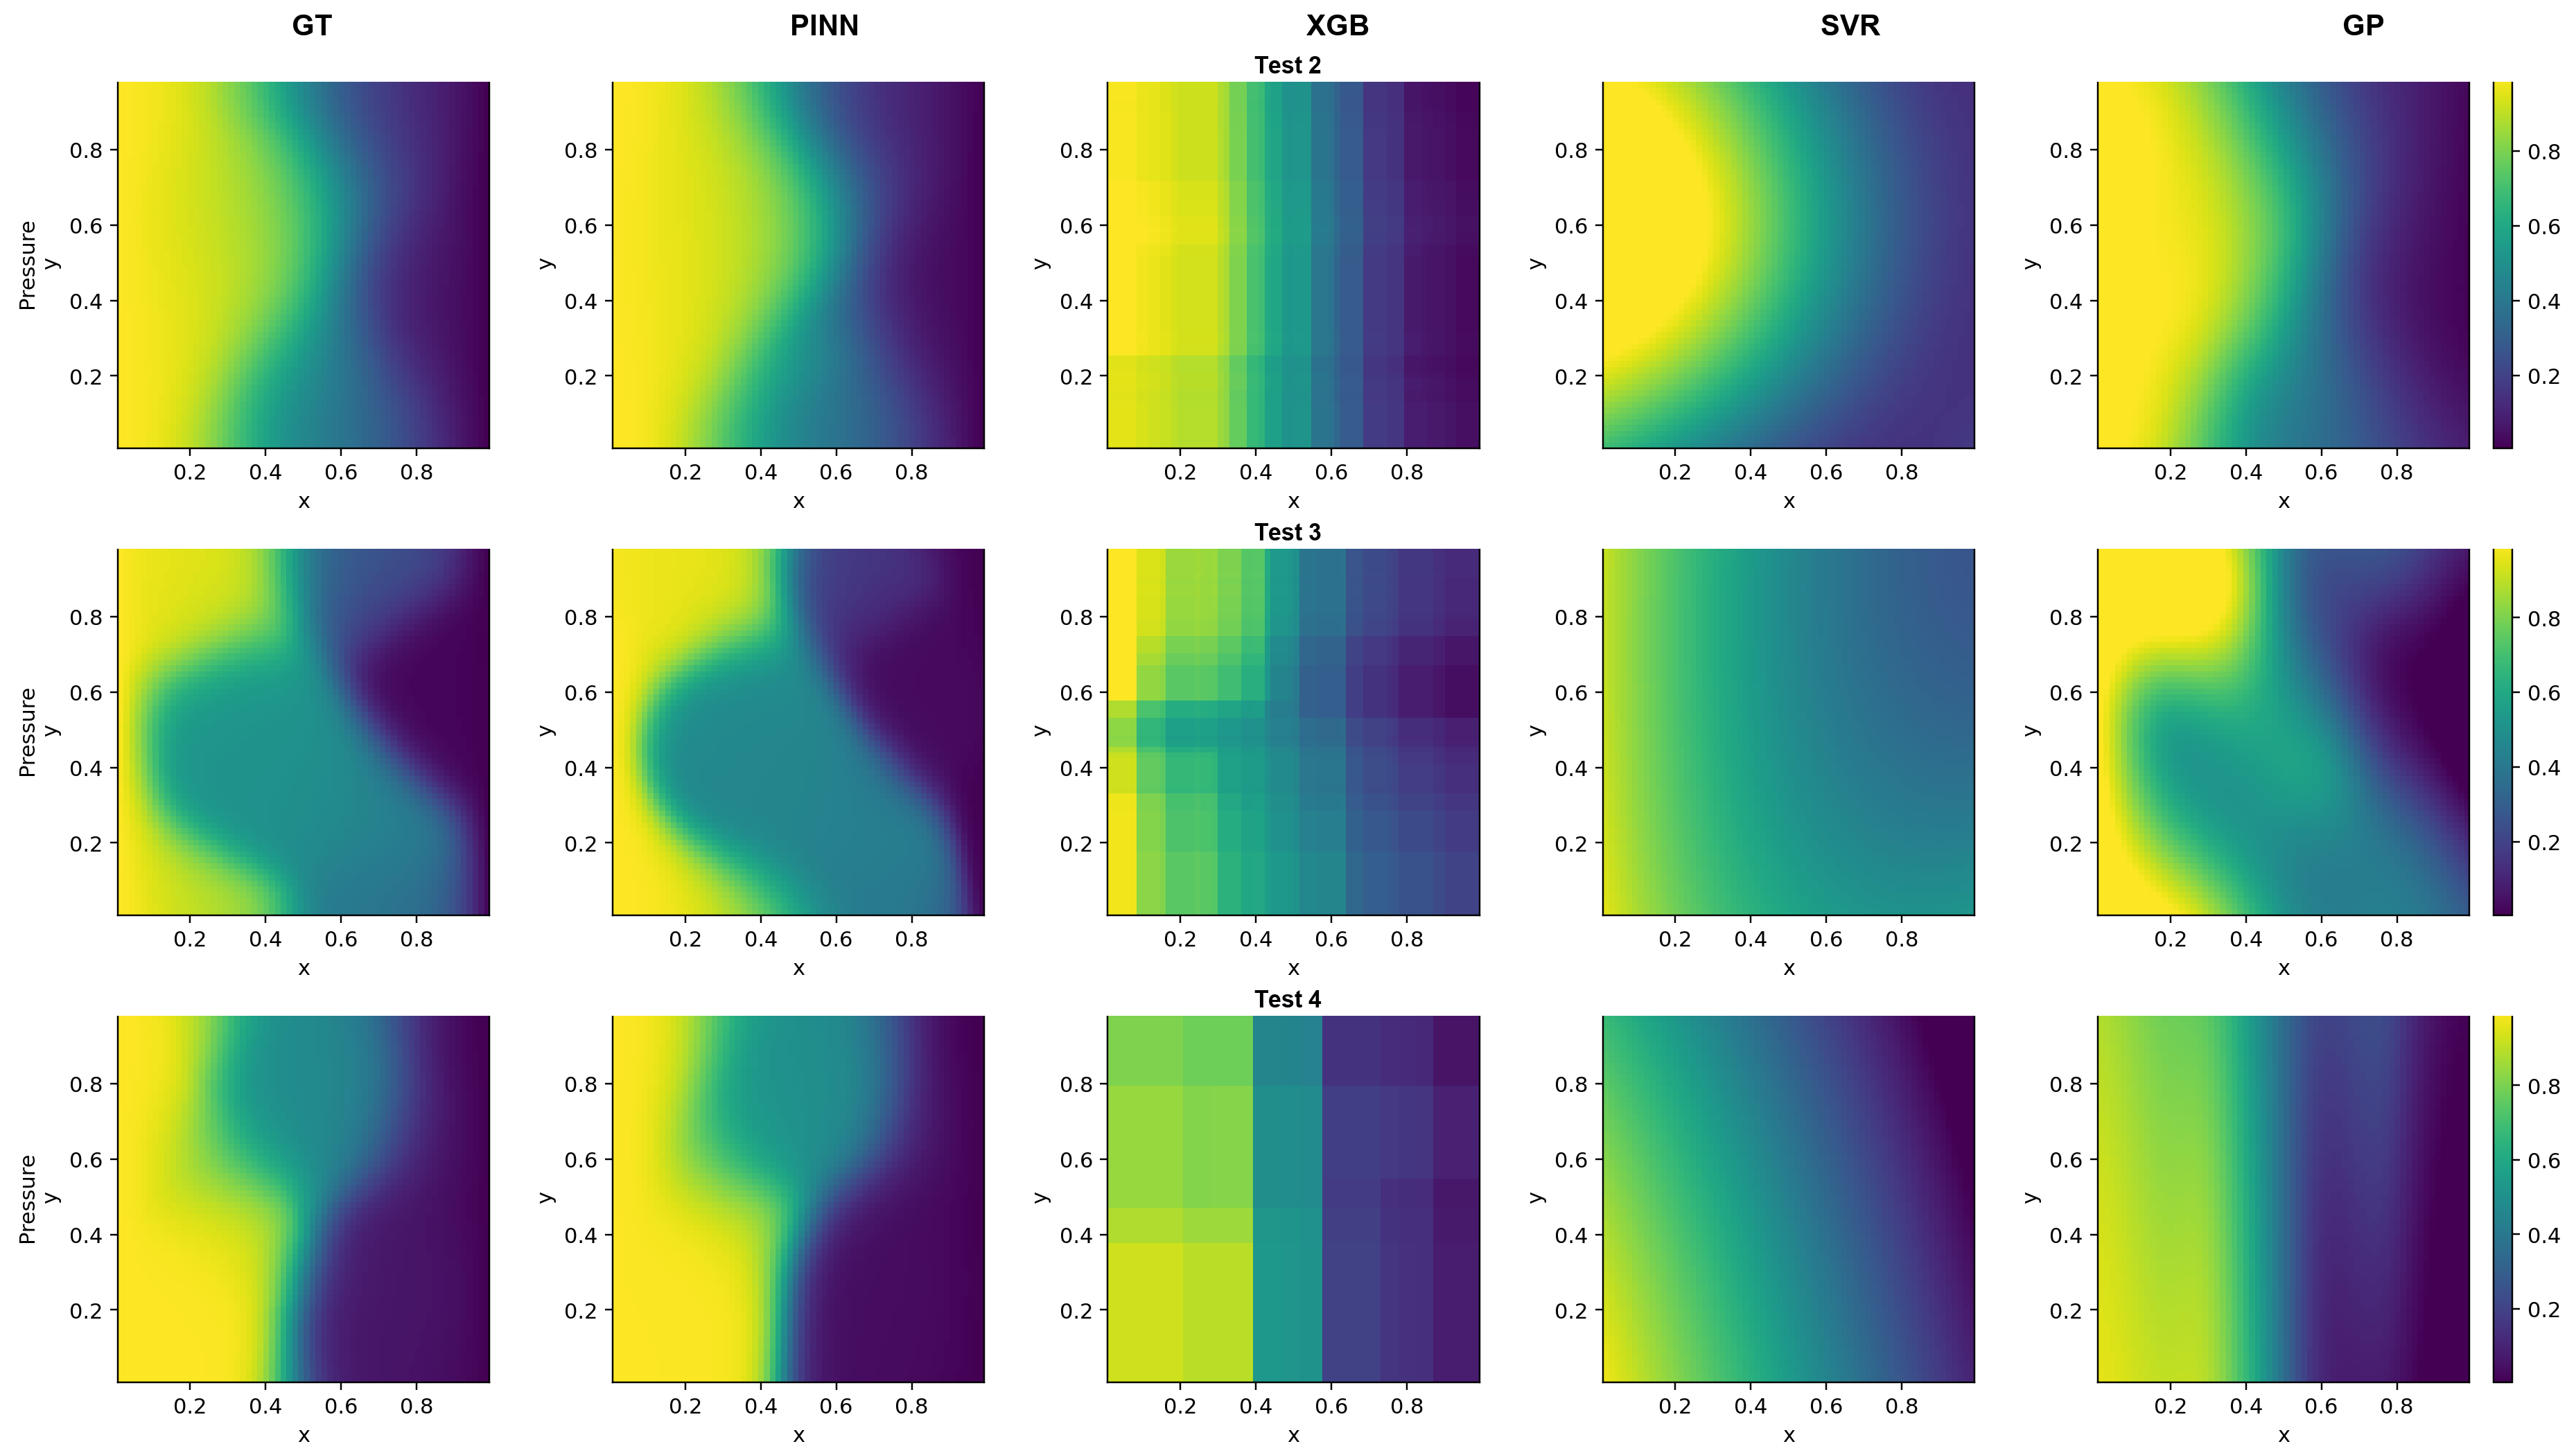
\includegraphics[width=0.94\textwidth]{qualitative_flow_pressure_composite.png}
\captionsetup{hypcap=false}
\captionof{figure}{Final forecasting-time pressure for seed 101. Rows show Tests 2--4; columns compare the reference, H-PINN, XGB, SVR, and GP. Tests 2 and 3 use \(N=50\); Test 4 uses \(N=20\) and parameter realization 7. Shared row-wise colour limits make the comparatively smooth pressure target directly comparable across methods.}
\label{fig:qual_flow_pressure}
\end{strip}

Pressure is smooth relative to transported saturation and is already close to saturated in the target-resolved scores of Table~\ref{tab:target_summary}. Figure~\ref{fig:qual_flow_pressure} confirms that all methods reproduce the dominant left-to-right trend, although XGB remains block-like and SVR suppresses heterogeneity. The visual comparison therefore supports reporting water saturation as the primary flow target rather than averaging it with the much easier pressure field.

\clearpage
\begin{table}[H]
\centering
\scriptsize
\setlength{\tabcolsep}{1.5pt}
\caption{Physical diagnostics in the forecasting region at $N=50$ (mean $\pm$ sample standard deviation). The violation rate is the fraction of predictions outside $[-10^{-3},1+10^{-3}]$ for either saturation; closure is $|\widehat S_w+\widehat S_o-1|$.}
\label{tab:physical_diagnostics}
\begin{tabular}{@{}llcc@{}}
\toprule
Test & Method & Violation rate & Closure MAE \\
\midrule
T2 & H & $0.0000\pm0.0000$ & $\num{9.59e-09}\pm\num{1.05e-09}$ \\
T2 & HO & $0.0000\pm0.0000$ & $\num{9.52e-09}\pm\num{3.61e-10}$ \\
T2 & XGB & $0.1231\pm0.0999$ & $\num{2.67e-02}\pm\num{7.93e-03}$ \\
T2 & SVR & $0.1858\pm0.1306$ & $\num{8.47e-03}\pm\num{6.24e-03}$ \\
T2 & GP & $0.0520\pm0.0747$ & $\num{2.14e-07}\pm\num{3.49e-07}$ \\
\addlinespace[1pt]
T3 & H & $0.0000\pm0.0000$ & $\num{1.02e-08}\pm\num{3.03e-09}$ \\
T3 & HO & $0.0000\pm0.0000$ & $\num{9.54e-09}\pm\num{2.42e-09}$ \\
T3 & XGB & $0.0527\pm0.0655$ & $\num{6.96e-02}\pm\num{3.09e-02}$ \\
T3 & SVR & $0.1573\pm0.0804$ & $\num{1.13e-02}\pm\num{9.49e-03}$ \\
T3 & GP & $0.0373\pm0.0419$ & $\num{1.75e-08}\pm\num{1.18e-08}$ \\
\addlinespace[1pt]
T4 & H & $0.0000\pm0.0000$ & $\num{8.09e-09}\pm\num{7.55e-10}$ \\
T4 & HO & $0.0000\pm0.0000$ & $\num{8.74e-09}\pm\num{1.11e-09}$ \\
T4 & XGB & $0.1078\pm0.1124$ & $\num{1.76e-02}\pm\num{2.83e-03}$ \\
T4 & SVR & $0.0133\pm0.0231$ & $\num{2.38e-03}\pm\num{2.06e-03}$ \\
T4 & GP & $0.0551\pm0.0512$ & $\num{1.32e-08}\pm\num{4.64e-09}$ \\
\bottomrule
\end{tabular}
\end{table}


\subsection{Computational cost}
Classical times include the complete target-wise hyperparameter search, while PINN times include automatic differentiation and checkpoint selection. Reference-solver generation is excluded for every surrogate because the same generated states define the common labelled pool.

\begin{table*}[!htbp]
\centering
\small
\setlength{\tabcolsep}{3.5pt}
\caption{Wall-clock fitting and tuning time in seconds at $N=50$ (mean $\pm$ sample standard deviation over three seeds). Classical times include hyperparameter selection; reference-data generation is excluded.}
\label{tab:runtime}
\begin{tabular}{lccccc}
\toprule
Test & H-PINN & HO-PINN & XGB & SVM & GP \\
\midrule
Test 1 & 134.52\,$\pm$\,18.86 & 216.36\,$\pm$\,31.72 & 0.30\,$\pm$\,0.00 & 0.08\,$\pm$\,0.00 & \textbf{0.07\,$\pm$\,0.02} \\
Test 2 & 279.91\,$\pm$\,68.78 & 417.58\,$\pm$\,42.82 & 4.48\,$\pm$\,0.45 & \textbf{0.61\,$\pm$\,0.03} & 3.20\,$\pm$\,0.16 \\
Test 3 & 229.22\,$\pm$\,21.09 & 447.80\,$\pm$\,160.06 & 4.05\,$\pm$\,0.38 & \textbf{0.62\,$\pm$\,0.01} & 5.63\,$\pm$\,0.27 \\
Test 4 & 287.82\,$\pm$\,79.38 & 421.88\,$\pm$\,73.71 & 4.57\,$\pm$\,0.43 & \textbf{0.56\,$\pm$\,0.01} & 7.74\,$\pm$\,2.40 \\
\bottomrule
\end{tabular}
\end{table*}

